% Created 2016-08-17 Wed 14:38
\documentclass[tikz]{standalone}

\usepackage{arrayjob}

\usepackage[utf8]{inputenc}
\usepackage[T1]{fontenc}
\usepackage{helvet}
\usepackage{../../templates/msc}

\renewcommand{\familydefault}{\sfdefault}

\tikzset{
every picture/.style={
line width=1pt
}}

\usepackage{tikz}
\author{Holger Karl}
\date{\today}
\title{}


\begin{document}

% state machine 



\newcommand{\mygraph}[1]{% 
  \foreach \pos/\vvalue/\col [count = \i] in { (-1,0)/17/white, 
       (0,3)/22/black, (0.5,1)/12/red, (2,1)/19/green, (3,3)/9/blue, 
       (3,0)/5/cyan, (4,2)/8/magenta, (5,1)/13/yellow} {
           \pgfmathsetmacro{\value}{{#1}[\i-1]} 
           \pgfmathsetmacro{\active}{{#1}[\i+7]} 
           \ifnum\active=0
           \node [circle, draw, thin, fill=\col!10] (\i)  at \pos {\value }; 
           \fi 
           \ifnum\active=1
           \node [circle, draw, very thick, fill=\col!10, label=above right:\emph{done}] (\i)  at \pos {\value }; 
           \fi            
           \ifnum\active>1
           \pgfmathsetmacro{\acks}{int(\active-3)} 
           \node [circle, draw, very thick, fill=\col!50, label=above right:\emph{\small \acks}] (\i)  at \pos {\value }; 
           \fi 
    }
    
   \foreach \ida/\idb   in {1/2, 1/3, 2/3, 3/4, 4/5, 4/6, 5/6, 5/7, 6/7, 6/8} {
     \draw [thin] (\ida) -- (\idb);
   }
}

\newcommand{\onearrow}[4]{
  % from, to, bend, label 
  \draw [->, shorten >= .1cm, shorten <= 0.1cm] (#1) to [bend #3=30] node [midway, auto] {#4}  (#2) ;   
}

\newcommand{\parents}[1]{
  \foreach \a/\b in {#1}
  \draw [->, very thick] (\a) -- (\b);
}


\begin{tikzpicture}
  \mygraph{1,2,3,4,5,6,7,8,0,0,0,0,0,0,0,0}
\end{tikzpicture}

\begin{tikzpicture}
  \mygraph{17,22,12,19,9,5,8,13,0,0,0,0,0,0,0,0}
\end{tikzpicture}


% status fields: 
% 0: idle, 1: done; >=2: awake with n-2 acks/nacks arrived 

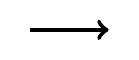
\begin{tikzpicture}
  \begin{scope}
    % Node 7 sends: 
    \mygraph{17,22,12,19,9,5,8,13,0,0,0,0,0,0,3,0} 
    \onearrow{7}{5}{right}{8}
    \onearrow{7}{6}{left}{8}
  \end{scope}
  \draw[ultra thick, ->] (6,1.5) -- (7,1.5);
  \begin{scope}[xshift=8cm]
    \mygraph{17,22,12,19,9,8,8,13,0,0,0,0,3,1,3,0}
    \parents{6/7}
  \end{scope}
\end{tikzpicture}

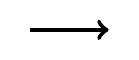
\begin{tikzpicture}
  \begin{scope}
    % Node 6 sends: 
    \mygraph{17,22,12,19,9,8,8,13,0,0,0,0,3,1,3,0}
    \parents{6/7}
    \onearrow{6}{5}{right}{8}
    \onearrow{6}{4}{left}{8}
    \onearrow{6}{8}{right}{8}
  \end{scope}
  \draw[ultra thick, ->] (6,1.5) -- (7,1.5);
  \begin{scope}[xshift=8cm]
    \mygraph{17,22,12,19,9,8,8,13,0,0,0,3,3,1,3,3}
    \parents{6/7}
  \end{scope}
\end{tikzpicture}

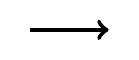
\begin{tikzpicture}
  \begin{scope}
    % Node 4 sends: 
    \mygraph{17,22,12,19,9,8,8,13,0,0,0,0,3,1,3,0}
    \parents{6/7}
    \onearrow{4}{3}{right}{19}
    \onearrow{4}{5}{left}{19}
    \onearrow{4}{6}{right}{19}
  \end{scope}
  \draw[ultra thick, ->] (6,1.5) -- (7,1.5);
  \begin{scope}[xshift=8cm]
    \mygraph{17,22,19,19,19,19,8,13,0,0,3,3,3,3,3,3}
    \parents{3/4,5/4,6/4}
  \end{scope}
\end{tikzpicture}

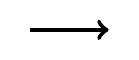
\begin{tikzpicture}
  \begin{scope}
    % Node 8 sends: 
    \mygraph{17,22,19,19,19,19,8,13,0,0,1,3,1,1,3,3}
    \parents{3/4,5/4,6/4}
    \onearrow{8}{6}{right}{13}
  \end{scope}
  \draw[ultra thick, ->] (6,1.5) -- (7,1.5);
  \begin{scope}[xshift=8cm]
    \mygraph{17,22,19,19,19,19,8,13,0,0,3,3,3,3,3,3}
    \parents{3/4,5/4,6/4}
  \end{scope}
\end{tikzpicture}


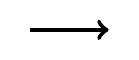
\begin{tikzpicture}
  \begin{scope}
    % Node 6 sends: 
    \mygraph{17,22,19,19,19,19,8,13,0,0,3,3,3,3,3,3}
    \parents{3/4,5/4,6/4}
    \onearrow{6}{5}{right}{19}
    \onearrow{6}{7}{right}{19}
    \onearrow{6}{8}{right}{19}
  \end{scope}
  \draw[ultra thick, ->] (6,1.5) -- (7,1.5);
  \begin{scope}[xshift=8cm]
    \mygraph{17,22,19,19,19,19,19,19,0,0,3,3,3,3,3,3}
    \parents{3/4,5/4,6/4,8/6,7/6}
  \end{scope}
\end{tikzpicture}

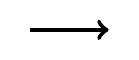
\begin{tikzpicture}
  \begin{scope}
    % Node 6 sends: 
    \mygraph{17,22,19,19,19,19,19,19,0,0,3,3,3,3,3,3}
    \parents{3/4,5/4,6/4,8/6,7/6}
    \onearrow{5}{6}{right}{NACK}
    \onearrow{8}{6}{left}{DONE}
  \end{scope}
  \draw[ultra thick, ->] (6,1.5) -- (7,1.5);
  \begin{scope}[xshift=8cm]
    \mygraph{17,22,19,19,19,19,19,19,0,0,3,3,3,5,3,1}
    \parents{3/4,5/4,6/4,8/6,7/6}
  \end{scope}
\end{tikzpicture}


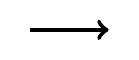
\begin{tikzpicture}
  \begin{scope}
    % Node 3 sends: 
    \mygraph{17,22,19,19,19,19,19,19,0,0,3,3,3,5,3,1}
    \parents{3/4,5/4,6/4,8/6,7/6}
    \onearrow{3}{2}{right}{19}
    \onearrow{3}{1}{left}{19}
  \end{scope}
  \draw[ultra thick, ->] (6,1.5) -- (7,1.5);
  \begin{scope}[xshift=8cm]
    \mygraph{19,22,19,19,19,19,19,19,3,3,3,3,3,5,3,1}
    \parents{1/3,3/4,5/4,6/4,8/6,7/6}
  \end{scope}
\end{tikzpicture}


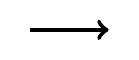
\begin{tikzpicture}
  \begin{scope}
    % Node 2 sends: 
    \mygraph{19,22,19,19,19,19,19,19,3,3,3,3,3,5,3,1}
    \parents{1/3,3/4,5/4,6/4,8/6,7/6}
    \onearrow{2}{1}{right}{22}
    \onearrow{2}{3}{left}{22}
  \end{scope}
  \draw[ultra thick, ->] (6,1.5) -- (7,1.5);
  \begin{scope}[xshift=8cm]
    \mygraph{22,22,22,19,19,19,19,19,3,3,3,3,3,5,3,1}
    \parents{1/2,3/2,5/4,6/4,8/6,7/6}
  \end{scope}
\end{tikzpicture}


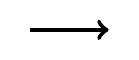
\begin{tikzpicture}
  \begin{scope}
    % Node 1 sends: 
    \mygraph{22,22,22,19,19,19,19,19,3,3,3,3,3,5,3,1}
    \parents{1/2,3/2,5/4,6/4,8/6,7/6}
    \onearrow{1}{3}{right}{22}
  \end{scope}
  \draw[ultra thick, ->] (6,1.5) -- (7,1.5);
  \begin{scope}[xshift=8cm]
    \mygraph{22,22,22,19,19,19,19,19,4,3,3,3,3,5,3,1}
    \onearrow{3}{1}{left}{NACK}
    \parents{1/2,3/2,5/4,6/4,8/6,7/6}
  \end{scope}
\end{tikzpicture}

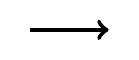
\begin{tikzpicture}
  \begin{scope}
    % Node 1 sends: 
    \mygraph{22,22,22,19,19,19,19,19,4,3,3,3,3,5,3,1}
    \parents{1/2,3/2,5/4,6/4,8/6,7/6}
    \onearrow{1}{2}{left}{DONE}
  \end{scope}
  \draw[ultra thick, ->] (6,1.5) -- (7,1.5);
  \begin{scope}[xshift=8cm]
    \mygraph{22,22,22,19,19,19,19,19,1,4,3,3,3,5,3,1}
    \parents{1/2,3/2,5/4,6/4,8/6,7/6}
  \end{scope}
\end{tikzpicture}

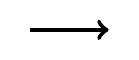
\begin{tikzpicture}
  \begin{scope}
    % Node 3 sends: 
    \mygraph{22,22,22,19,19,19,19,19,1,4,3,3,3,5,3,1}
    \parents{1/2,3/2,5/4,6/4,8/6,7/6}
    \onearrow{3}{1}{left}{22}
    \onearrow{3}{4}{left}{22}
  \end{scope}
  \draw[ultra thick, ->] (6,1.5) -- (7,1.5);
  \begin{scope}[xshift=8cm]
    \mygraph{22,22,22,22,19,19,19,19,1,4,4,3,3,5,3,1}
    \onearrow{1}{3}{left}{NACK}
    \parents{1/2,3/2,4/3,5/4,6/4,8/6,7/6}
  \end{scope}
\end{tikzpicture}

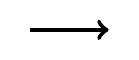
\begin{tikzpicture}
  \begin{scope}
    % Node 4 sends: 
    \mygraph{22,22,22,22,19,19,19,19,1,4,4,3,3,5,3,1}
    \parents{1/2,3/2,4/3,5/4,6/4,8/6,7/6}
    \onearrow{4}{5}{left}{22}
    \onearrow{4}{6}{right}{22}
  \end{scope}
  \draw[ultra thick, ->] (6,1.5) -- (7,1.5);
  \begin{scope}[xshift=8cm]
    \mygraph{22,22,22,22,22,22,19,19,1,4,4,3,3,3,3,1}
    \parents{1/2,3/2,4/3,5/4,6/4,8/6,7/6}
  \end{scope}
\end{tikzpicture}

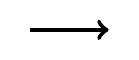
\begin{tikzpicture}
  \begin{scope}
    % Node 6 sends: 
    \mygraph{22,22,22,22,22,22,19,19,1,4,4,3,3,3,3,1}
    \parents{1/2,3/2,4/3,5/4,6/4,8/6,7/6}
    \onearrow{6}{5}{right}{22}
    \onearrow{6}{7}{right}{22}
    \onearrow{6}{8}{right}{22}
  \end{scope}
  \draw[ultra thick, ->] (6,1.5) -- (7,1.5);
  \begin{scope}[xshift=8cm]
    \mygraph{22,22,22,22,22,22,22,22,1,4,4,3,3,5,3,1}
    \parents{1/2,3/2,4/3,5/4,6/4,8/6,7/6}
    \onearrow{8}{6}{right}{DONE}
    \onearrow{5}{6}{left}{NACK}
  \end{scope}
\end{tikzpicture}

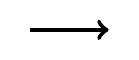
\begin{tikzpicture}
  \begin{scope}
    % Node 6 sends: 
    \mygraph{22,22,22,22,22,22,19,19,1,4,4,3,3,3,3,1}
    \parents{1/2,3/2,4/3,5/4,6/4,8/6,7/6}
    \onearrow{6}{5}{right}{22}
    \onearrow{6}{7}{right}{22}
    \onearrow{6}{8}{right}{22}
  \end{scope}
  \draw[ultra thick, ->] (6,1.5) -- (7,1.5);
  \begin{scope}[xshift=8cm]
    \mygraph{22,22,22,22,22,22,22,22,1,4,4,3,4,5,3,1}
    \parents{1/2,3/2,4/3,5/4,6/4,8/6,7/6}
    \onearrow{8}{6}{right}{DONE}
    \onearrow{5}{6}{left}{NACK}
  \end{scope}
\end{tikzpicture}

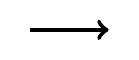
\begin{tikzpicture}
  \begin{scope}
    % Node 5 sends: 
    \mygraph{22,22,22,22,22,22,22,22,1,4,4,3,4,5,3,1}
    \parents{1/2,3/2,4/3,5/4,6/4,8/6,7/6}
    \onearrow{5}{7}{left}{22}
  \end{scope}
  \draw[ultra thick, ->] (6,1.5) -- (7,1.5);
  \begin{scope}[xshift=8cm]
    \mygraph{22,22,22,22,22,22,22,22,1,4,4,3,5,5,3,1}
    \parents{1/2,3/2,4/3,5/4,6/4,8/6,7/6}
    \onearrow{7}{5}{right}{NACK}
  \end{scope}
\end{tikzpicture}

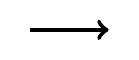
\begin{tikzpicture}
  \begin{scope}
    % Node 5 sends: 
    \mygraph{22,22,22,22,22,22,22,22,1,4,4,3,4,5,3,1}
    \parents{1/2,3/2,4/3,5/4,6/4,8/6,7/6}
    \onearrow{5}{4}{right}{DONE}
  \end{scope}
  \draw[ultra thick, ->] (6,1.5) -- (7,1.5);
  \begin{scope}[xshift=8cm]
    \mygraph{22,22,22,22,22,22,22,22,1,4,4,4,5,5,3,1}
    \parents{1/2,3/2,4/3,5/4,6/4,8/6,7/6}
  \end{scope}
\end{tikzpicture}

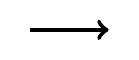
\begin{tikzpicture}
  \begin{scope}
    % Node 7 sends: 
    \mygraph{22,22,22,22,22,22,22,22,1,4,4,4,5,5,3,1}
    \parents{1/2,3/2,4/3,5/4,6/4,8/6,7/6}
    \onearrow{7}{5}{right}{22}
  \end{scope}
  \draw[ultra thick, ->] (6,1.5) -- (7,1.5);
  \begin{scope}[xshift=8cm]
    \mygraph{22,22,22,22,22,22,22,22,1,4,4,4,1,5,5,1}
    \parents{1/2,3/2,4/3,5/4,6/4,8/6,7/6}
    \onearrow{5}{7}{left}{DONE}
  \end{scope}
\end{tikzpicture}

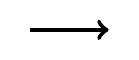
\begin{tikzpicture}
  \begin{scope}
    % Node 7 sends: 
    \mygraph{22,22,22,22,22,22,22,22,1,4,4,4,1,5,1,1}
    \parents{1/2,3/2,4/3,5/4,6/4,8/6,7/6}
    \onearrow{7}{6}{left}{DONE}
  \end{scope}
  \draw[ultra thick, ->] (6,1.5) -- (7,1.5);
  \begin{scope}[xshift=8cm]
    \mygraph{22,22,22,22,22,22,22,22,1,4,4,4,1,6,1,1}
    \parents{1/2,3/2,4/3,5/4,6/4,8/6,7/6}
  \end{scope}
\end{tikzpicture}

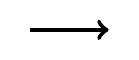
\begin{tikzpicture}
  \begin{scope}
    % Node 7 sends: 
    \mygraph{22,22,22,22,22,22,22,22,1,4,4,4,1,1,1,1}
    \parents{1/2,3/2,4/3,5/4,6/4,8/6,7/6}
    \onearrow{6}{4}{left}{DONE}
  \end{scope}
  \draw[ultra thick, ->] (6,1.5) -- (7,1.5);
  \begin{scope}[xshift=8cm]
    \mygraph{22,22,22,22,22,22,22,22,1,4,4,5,1,1,1,1}
    \parents{1/2,3/2,4/3,5/4,6/4,8/6,7/6}
  \end{scope}
\end{tikzpicture}

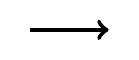
\begin{tikzpicture}
  \begin{scope}
    % Node 7 sends: 
    \mygraph{22,22,22,22,22,22,22,22,1,4,4,1,1,1,1,1}
    \parents{1/2,3/2,4/3,5/4,6/4,8/6,7/6}
    \onearrow{4}{3}{left}{DONE}
  \end{scope}
  \draw[ultra thick, ->] (6,1.5) -- (7,1.5);
  \begin{scope}[xshift=8cm]
    \mygraph{22,22,22,22,22,22,22,22,1,4,5,1,1,1,1,1}
    \parents{1/2,3/2,4/3,5/4,6/4,8/6,7/6}
  \end{scope}
\end{tikzpicture}

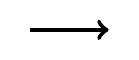
\begin{tikzpicture}
  \begin{scope}
    % Node 3 sends: 
    \mygraph{22,22,22,22,22,22,22,22,1,4,1,1,1,1,1,1}
    \parents{1/2,3/2,4/3,5/4,6/4,8/6,7/6}
    \onearrow{3}{2}{left}{DONE}
  \end{scope}
  \draw[ultra thick, ->] (6,1.5) -- (7,1.5);
  \begin{scope}[xshift=8cm]
    \mygraph{22,22,22,22,22,22,22,22,1,5,1,1,1,1,1,1}
    \parents{1/2,3/2,4/3,5/4,6/4,8/6,7/6}
  \end{scope}
\end{tikzpicture}
\begin{tikzpicture}
  \begin{scope}
    % Node 3 sends: 
    \mygraph{22,22,22,22,22,22,22,22,1,5,1,1,1,1,1,1}
    \parents{1/2,3/2,4/3,5/4,6/4,8/6,7/6}
    \node [star, draw, fill=red] at (0.5,3.5) {};     
  \end{scope}
\end{tikzpicture}

\end{document}